\documentclass[paper=a4, fontsize=10pt]{scrartcl} % A4 paper and 11pt font size

\usepackage[T1]{fontenc} % Use 8-bit encoding that has 256 glyphs
\usepackage{fourier} % Use the Adobe Utopia font for the document - comment this line to return to the LaTeX default
\usepackage[english]{babel} % English language/hyphenation
\usepackage{amsmath,amsfonts,amsthm} % Math packages
\usepackage{graphicx}
\usepackage[cm]{fullpage}
\usepackage{float}
\usepackage{sectsty} % Allows customizing section commands
\allsectionsfont{\centering \normalfont\scshape} % Make all sections centered, the default font and small caps

\usepackage{fancyhdr} % Custom headers and footers
\pagestyle{fancyplain} % Makes all pages in the document conform to the custom headers and footers
\fancyhead{} % No page header - if you want one, create it in the same way as the footers below
\fancyfoot[L]{} % Empty left footer
\fancyfoot[C]{} % Empty center footer
\fancyfoot[R]{\thepage} % Page numbering for right footer
\renewcommand{\headrulewidth}{0pt} % Remove header underlines
\renewcommand{\footrulewidth}{0pt} % Remove footer underlines
\setlength{\headheight}{13.6pt} % Customize the height of the header

\numberwithin{equation}{section} % Number equations within sections (i.e. 1.1, 1.2, 2.1, 2.2 instead of 1, 2, 3, 4)
\numberwithin{figure}{section} % Number figures within sections (i.e. 1.1, 1.2, 2.1, 2.2 instead of 1, 2, 3, 4)
\numberwithin{table}{section} % Number tables within sections (i.e. 1.1, 1.2, 2.1, 2.2 instead of 1, 2, 3, 4)

\setlength\parindent{0pt} % Removes all indentation from paragraphs - comment this line for an assignment with lots of text

%----------------------------------------------------------------------------------------
%	TITLE SECTION
%----------------------------------------------------------------------------------------

\newcommand{\horrule}[1]{\rule{\linewidth}{#1}} % Create horizontal rule command with 1 argument of height

\newtoks\rowvectoks
\newcommand{\rowvec}[2]{%
  \rowvectoks={#2}\count255=#1\relax
  \advance\count255 by -1
  \rowvecnexta}
\newcommand{\rowvecnexta}{%
  \ifnum\count255>0
    \expandafter\rowvecnextb
  \else
    \begin{pmatrix}\the\rowvectoks\end{pmatrix}
  \fi}
\newcommand\rowvecnextb[1]{%
    \rowvectoks=\expandafter{\the\rowvectoks&#1}%
    \advance\count255 by -1
    \rowvecnexta}

\title{	
\normalfont \normalsize 
\textsc{Radboud University Nijmegen}  % Your university, school and/or department name(s)
\horrule{0.5pt} \\[0.3cm] % Thin top horizontal rule
\huge Statistical Machine Learning \\ Assignment 3 \\ % The assignment title
\horrule{2pt}  % Thick bottom horizontal rule
}

\author{Steven Reitsma \\ (s4132343)} % Your name

\date{\normalsize\today} % Today's date or a custom date

\begin{document}

\maketitle % Print the title

\section{Bayesian linear regression}
\begin{enumerate}
	\item   We follow the same procedure as in exercise 2, week 7, but we fill in the data points right away.

			\textbf{Step 1: Finding the vector $\phi(x)$}
			\begin{align}
				y(x, \boldsymbol w) &= \phi(\boldsymbol x)^T\boldsymbol w = w_0 + w_1x\\
				\phi(x) &= \begin{pmatrix}
								1\\
								x
							\end{pmatrix}
			\end{align}

			\textbf{Step 2: Write out $\Phi^T\boldsymbol t$ and $\Phi^T\Phi$ in terms of the data points}
			\begin{align}
				\Phi_{nj} &= \phi_j(x_n)\\
				\Phi &= \begin{pmatrix}
							1 & 0.4 \\
							1 & 0.6
						\end{pmatrix}\\
				\Phi^T \boldsymbol t &= \begin{pmatrix}
											1 & 1\\
											0.4 & 0.6
										\end{pmatrix}
										\begin{pmatrix}
											0.05\\
											-0.35
										\end{pmatrix}\\
									&= \begin{pmatrix}
											-0.3\\
											-0.19
										\end{pmatrix}\\
				\Phi^T\Phi &= \begin{pmatrix}
								1 & 1\\
								0.4 & 0.6
							 \end{pmatrix}
							 \begin{pmatrix}
							 	1 & 0.4\\
							 	1 & 0.6
							 \end{pmatrix}\\
							 &= \begin{pmatrix}
							 		2 & 1\\
							 		1 & 0.52
							 	\end{pmatrix}
			\end{align}

			\textbf{Step 3: Compute the posterior}
			\begin{align}
				p(\boldsymbol w \vert \boldsymbol t, \boldsymbol x) &= \mathcal{N}(\boldsymbol w \vert \boldsymbol m_N, \boldsymbol S_N)\\
				\boldsymbol m_N &= \beta \boldsymbol S_N \Phi^T \boldsymbol t\\
				\boldsymbol S_N^{-1} &= \alpha \boldsymbol I + \beta \Phi^T\Phi\\
								 &= \begin{pmatrix}
								 		\alpha & 0\\
								 		0 & \alpha
								 	\end{pmatrix} + 
								 	\beta \begin{pmatrix}
								 				2 & 1\\
								 				1 & 0.52
								 		  \end{pmatrix}\\
				\alpha &= 2\\
				\beta &= 10\\
				\boldsymbol S_N^{-1} &= \begin{pmatrix}
											22 & 10\\
											10 & 7.2
										  \end{pmatrix}\\
				\boldsymbol m_N &= 10 \begin{pmatrix}
											22 & 10\\
											10 & 7.2
										\end{pmatrix}^{-1}
										\begin{pmatrix}
											-0.3\\
											-0.19
										\end{pmatrix}\\
								 &= \begin{pmatrix}
								 		-0.0445\\
								 		-0.2021
								 	\end{pmatrix}
			\end{align}

			\textbf{Step 4: Compute the predictive distribution}
			\begin{align}
				p(t \vert x, \boldsymbol t, \boldsymbol x) &= \mathcal{N}(t \vert \boldsymbol m_N^T \phi(x), \sigma^2_N(x))\\
														   &= \mathcal{N}(t \vert m(x), s^2(x))\\
				m(x) &= \boldsymbol m_N^T\phi(x) \\
				s^2(x) &= \sigma^2_N(x) = \frac{1}{\beta} + \phi(x)^T \boldsymbol S_N \phi(x)\\
				m(x) &= \begin{pmatrix}
							-0.0445\\
							-0.2021
						\end{pmatrix}^T
						\begin{pmatrix}
							1\\
							x
						\end{pmatrix}\\
				s^2(x) &= \frac{1}{10} + \begin{pmatrix}
											1\\
											x
										 \end{pmatrix}^T
										 \begin{pmatrix}
										 	22 & 10\\
										 	10 & 7.2
										 \end{pmatrix}^{-1}
										 \begin{pmatrix}
										 	1\\
										 	x
										 \end{pmatrix}
			\end{align}
	\item The plot is shown in figure \ref{meanvar}. The figure clearly shows that currently, the initial prior still has a large effect. In a maximum likelihood solution, the line would now go through both of the data points. This can be shown by taking a lower value of $\alpha$ (or taking higher $\beta$), which will decrease the prior's certainty. The difference with the figure 3.8b in Bishop is explained by the fact that we use only a two-dimensional Gaussian basis function $\phi_j$, whereas Bishop uses 9.

		  \begin{figure}[H]
			\centering
			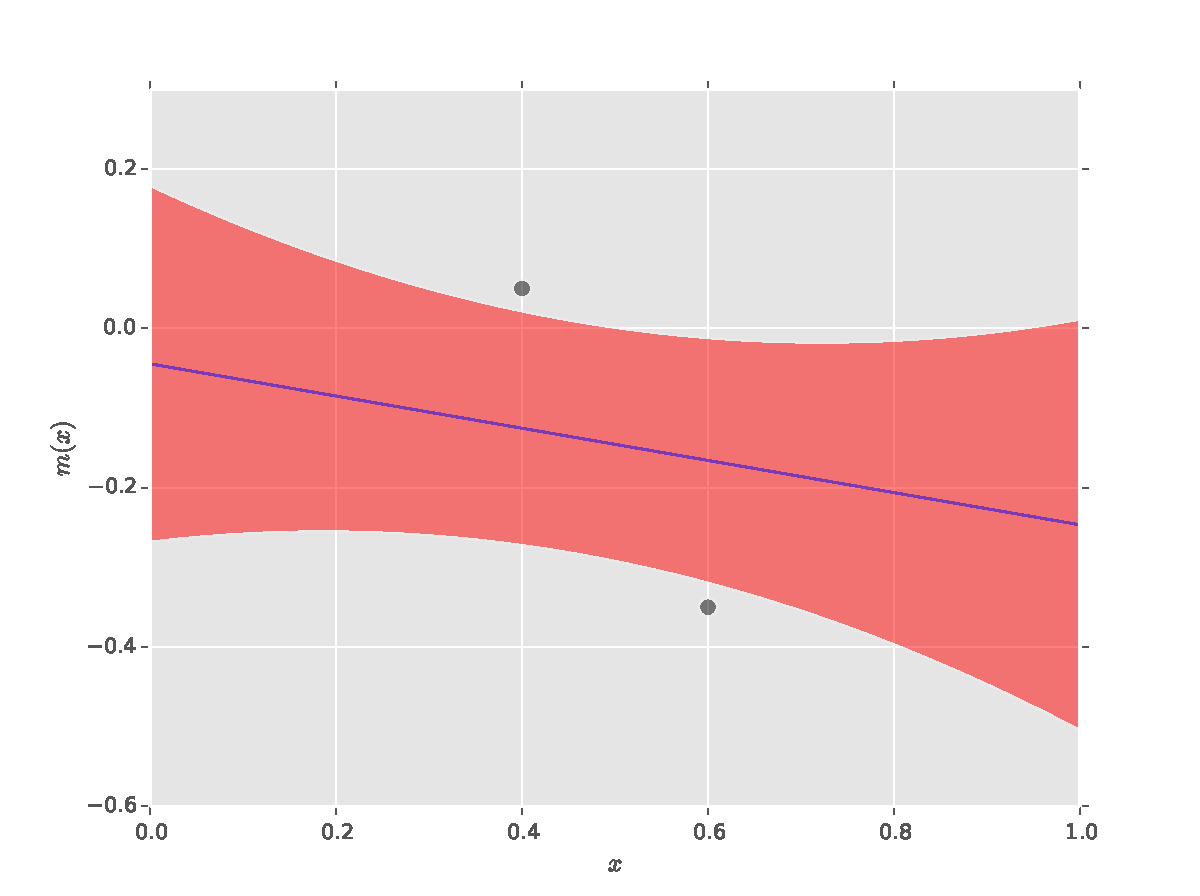
\includegraphics[scale=0.65]{exercise_12.pdf}
			\caption{The blue line indicates the mean of the predictive distribution plotted against x. The two gray dots are the data points and the red area indicates the standard deviation. The area is bound by the mean plus the standard deviation and by the mean minus the standard deviation.}
			\label{meanvar}
		  \end{figure}
	\item In figure \ref{sampled} some sampled linear equations are shown in green.

	\begin{figure}[H]
			\centering
			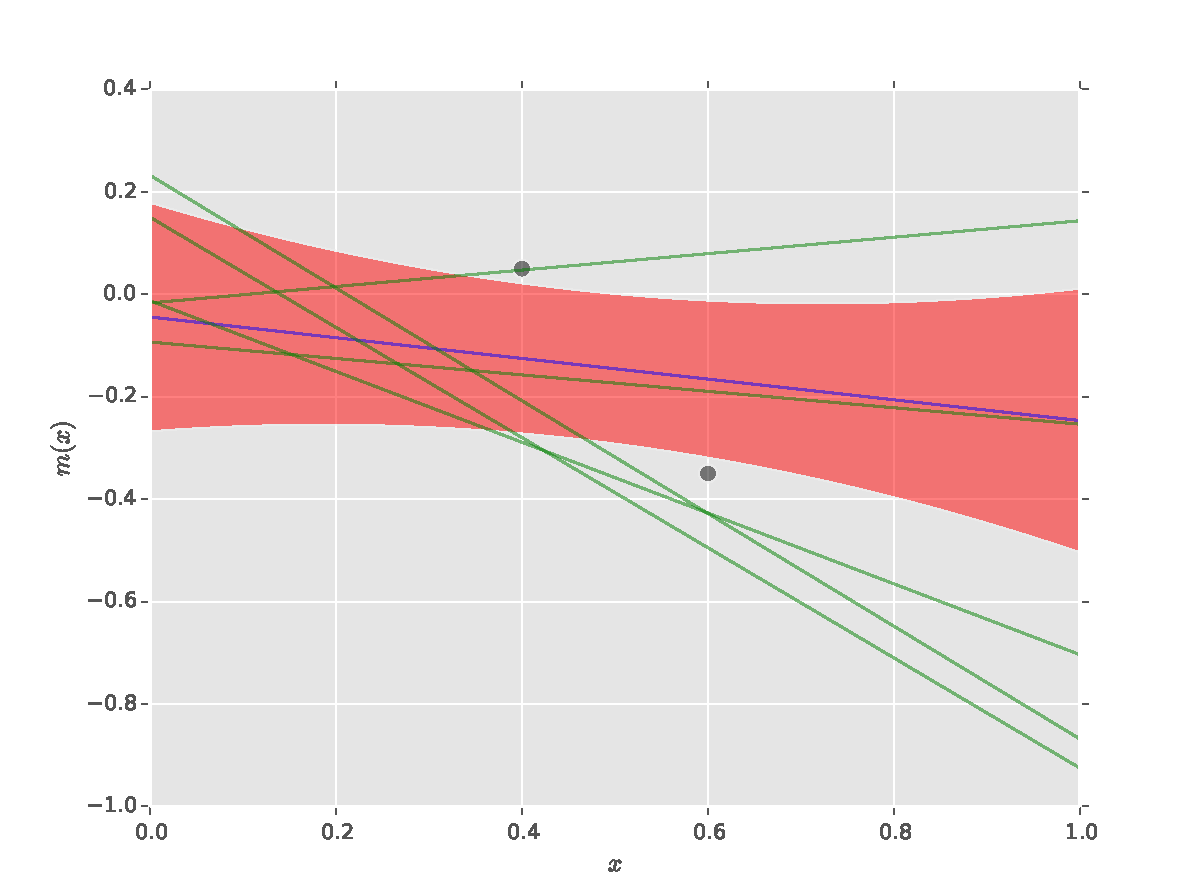
\includegraphics[scale=0.65]{exercise_13.pdf}
			\caption{The green lines represent $y(x, \boldsymbol w)$ where the weights $\boldsymbol w$ are sampled from the posterior distribution.}
			\label{sampled}
		  \end{figure}
\end{enumerate}

\section{Logistic regression}
\subsection{The IRLS algorithm}
\begin{enumerate}
	\item 
	\item
\end{enumerate}

\subsection{Two-class classification using logistic regression}
\begin{enumerate}
	\item 
	\item
	\item
	\item
	\item
\end{enumerate}

\end{document}